\chapter{Related Work}
\label{cha:related_work}
In this chapter, we present related work of this thesis. In section~\ref{sec:other_simulators}, we describe alternatives to Gazebo and why we choose Gazebo. In section~\ref{sec:simulations}, we give an overview of other popular simulations, especially a simulation that also uses Gazebo and other multi-robot simulations. Section~\ref{sec:multi_agent_strategies} describes our current multi-robot strategy as well as other attractive strategies our simulation should be able to evaluate. In the following, we will use the terms \textit{multi-robot} and \textit{multi-agent} interchangeably because both terms appear in the related work and are closely related to each other. A multi-agent system can consist of fully abstract agents and a multi-robot system is a multi-agent system with robotic agents that interact physically with their environment.


\section{Robot Simulators}
\label{sec:other_simulators}
Robot simulators have become important tools in the development of robot software. In this section, we present some popular robot simulators and describe why we chose Gazebo.

\subsection{Stage}
\textit{Stage}\footnote{\url{https://github.com/rtv/Stage}} is an Open Source multi-robot simulator for a two dimensional environment. It is a part of the \textit{Player/Stage} project~\cite{{PlayerStage}}. \textit{Player} is a robot control server, which provides a simple connection between a robot control program, sensors and actuators of a robot. Stage uses this connection and replaces the sensors and actuators by simulated ones. Stage was a popular simulator in the last years and is able to simulate a large amount of robots. For the simulation, Stage uses simple models, which need little computational effort and provide enough fidelity for many applications. Furthermore, the computational effort is linear in the number of robots. Because of that, Stage can simulate a large amount of robots~\cite{stage_massive}. This makes Stage well suited for the simulation of swarms and multi-robot systems with many robots. However, the restriction to two dimensions is a problem for the use of Stage in this thesis. We want to simulate vision components to be able to test our system as a whole and under more realistic conditions. We also want to be extendable for future changes of LLSF or the use of the simulator in another domain, such as the RoboCup@Home league.

\subsection{Webots}
\textit{Webots}\footnote{\url{http://www.cyberbotics.com}} is a commercial 3D simulator~\cite{{Webots}}. It is platform independent and features a whole development environment for robot software including an editor and an API for inter-robot communication. Webots supports many programming languages and several standard robots and sensors out of the box. It is also able to simulate multiple robots and provides an interface for ROS and Matlab. Webots was used in a RoboCup Soccer simulation~\cite{webots_robocup}. Webots is no good choice for this thesis because it is commercial and no Open Source software. Therefore, it can be difficult to expand the simulation to our needs.

\subsection{USARSim}
\textit{USARSim}\footnote{\url{http://sourceforge.net/projects/usarsim}} is a 3D simulator developed for urban search and rescue scenarios~\cite{USARSim}. It has evolved to be able to simulate other domains too. Therefore, the abbreviation USARSim now stands for ``Unified System for Automation 
and Robotics Simulation'' instead of the previous ``Urban Search and Rescue Simulation''~\cite{USARSim}. It is platform independent and free of charge for research and education. The advantages of USARSim are the graphical realism of the Unreal engine\footnote{\url{http://www.unrealengine.com/udk}} and the physical realism by the PhysX engine\footnote{\url{https://developer.nvidia.com/physx}}. USARSim also provides an interface to ROS~\cite{USARSimROS} and is able to simulate multiple robots. It is used as a basis for the RoboCup Rescue Simulation League we also present in section 3.2.2.

\subsection{SimSpark}
\textit{SimSpark}\footnote{\url{http://simspark.sourceforge.net}} is an Open Source 3D simulator~\cite{simspark_old}. It was developed by the RoboCup community for the RoboCup 3D Soccer Simulation and has been used there since 2004. Therefore SimSpark is able to simulate multiple robots and specialized on the NAO as soccer robot. There are several improvements and new features of SimSpark~\cite{SimSpark,Visualization}, such as visualization of agent intentions, realistic servo motors for the NAO and better support of heterogeneous robot teams. Because Simspark and the community behind are mostly specialized on the RoboCup Soccer Simulation, it is not the best choice for this thesis.

\subsection{Robotino Sim Professional}
\textit{Robotino Sim Professional}\footnote{\url{http://www.festo-didactic.com/int-en/learning-systems/software-e-learning/robotino-sim-view/robotino-sim-professional.htm}} is a 3D simulator for the Robotino developed by its manufacturer Festo. It can be used to create and simulate environments made for the Robotino. It is a commercial software and only usable on Microsoft Windows. Furthermore, it is limited to the Robotino and the default sensors the Robotino is shipped with. Therefore, Robotino Sim Professional is no good choice for this thesis.

\subsection{Choice for Gazebo}
There are a couple of reasons why we chose Gazebo. First, it fits to our needs for a realistic simulator which can simulate the LLSF and supports a variety of features. It is extendable, used in a large variety of domains and has a big community. Gazebo is also well funded by the Open Source Robotics Foundation\footnote{\url{http://osrfoundation.org}} and Willow Garage\footnote{\url{http://www.willowgarage.com}} and there are also many plans to develop Gazebo further\footnote{\url{http://gazebosim.org/wiki/Roadmap}}. Therefore, Gazebo is likely to become even more important in the future.\\
Another important argument for Gazebo is that it was used at KBSG before as a simulator for MSL~\cite{MultiLevelAbstraction} and for scene reconstruction for fault analysis~\cite{KlingenDA}. We will present both applications later in this chapter.\\
There are only few disadvantages of Gazebo. A disadvantage is that Gazebo cannot handle a large amount of robots. The complexity of the simulations limits the simulation speed when using multiple robots. The number of robots to simulate at a reasonable speed is in the order of ten~\cite{GazeboDesign}. This can become a problem if the simulation runs on a slow computer or there are more robots to simulate at the same time. However, these disadvantages have a small impact on this thesis because we use only three robots in the LLSF.

\section{Applications of Robot Simulators}
\label{sec:simulations}
In this section, we present some applications of robot simulators that are related to this thesis. We present the Virtual Robotics Challenge as another simulation with Gazebo, some RoboCup simulations because of their focus on multi-robot systems and a scene reconstruction and MSL simulator as previous projects with Gazebo at the KBSG.

\subsection{Virtual Robotics Challenge}
\begin{figure}
  \centering
  \begin{subfigure}[b]{0.3\textwidth}
    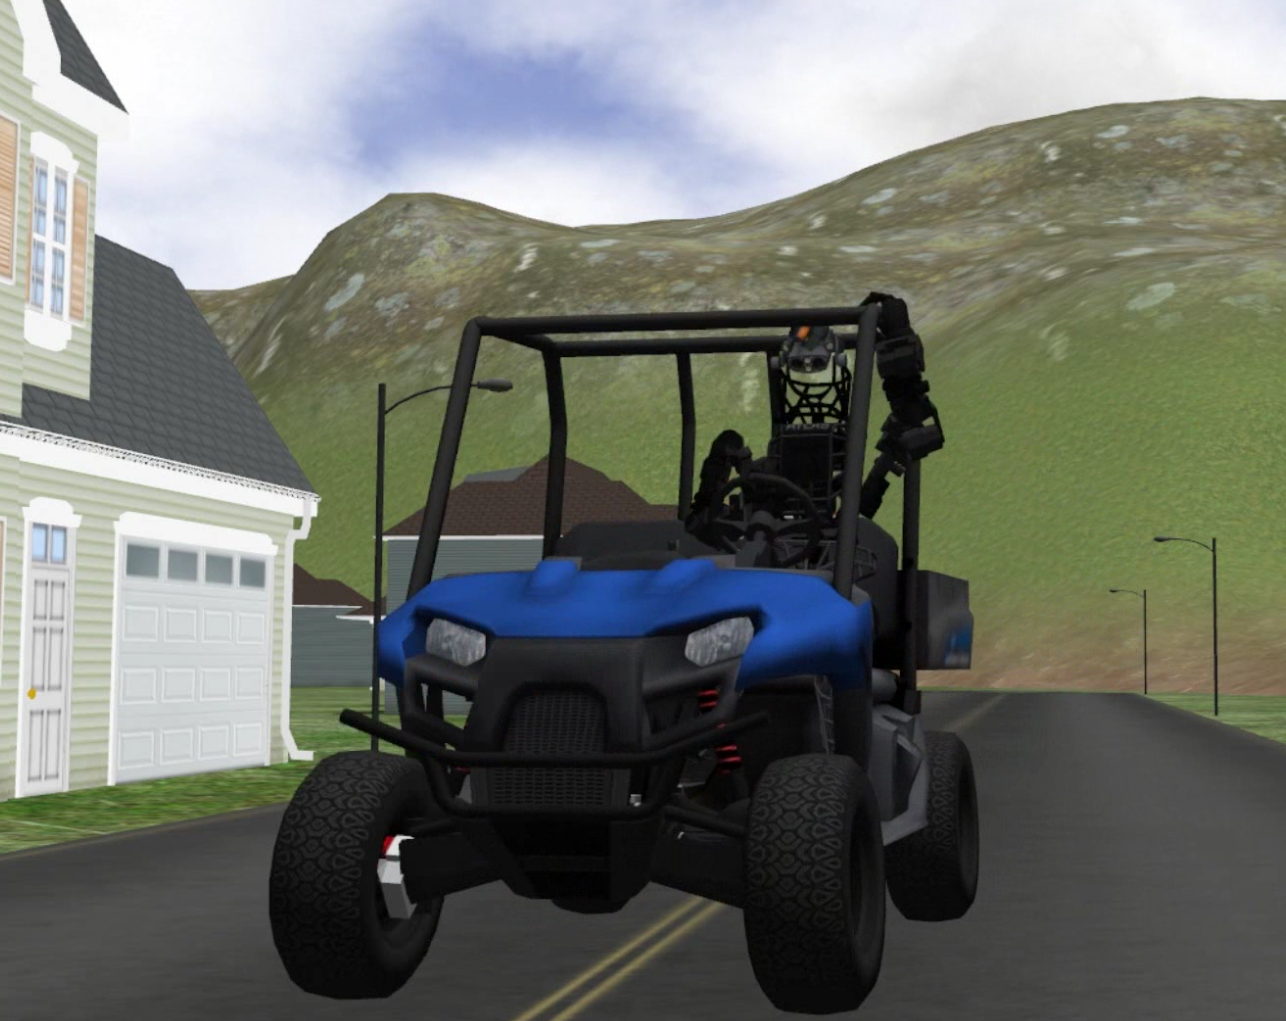
\includegraphics[width=\textwidth]{pics/darpa_car}
    \caption{Driving a car}
    \label{fig:vrc_car}
  \end{subfigure}
  \begin{subfigure}[b]{0.3\textwidth}
    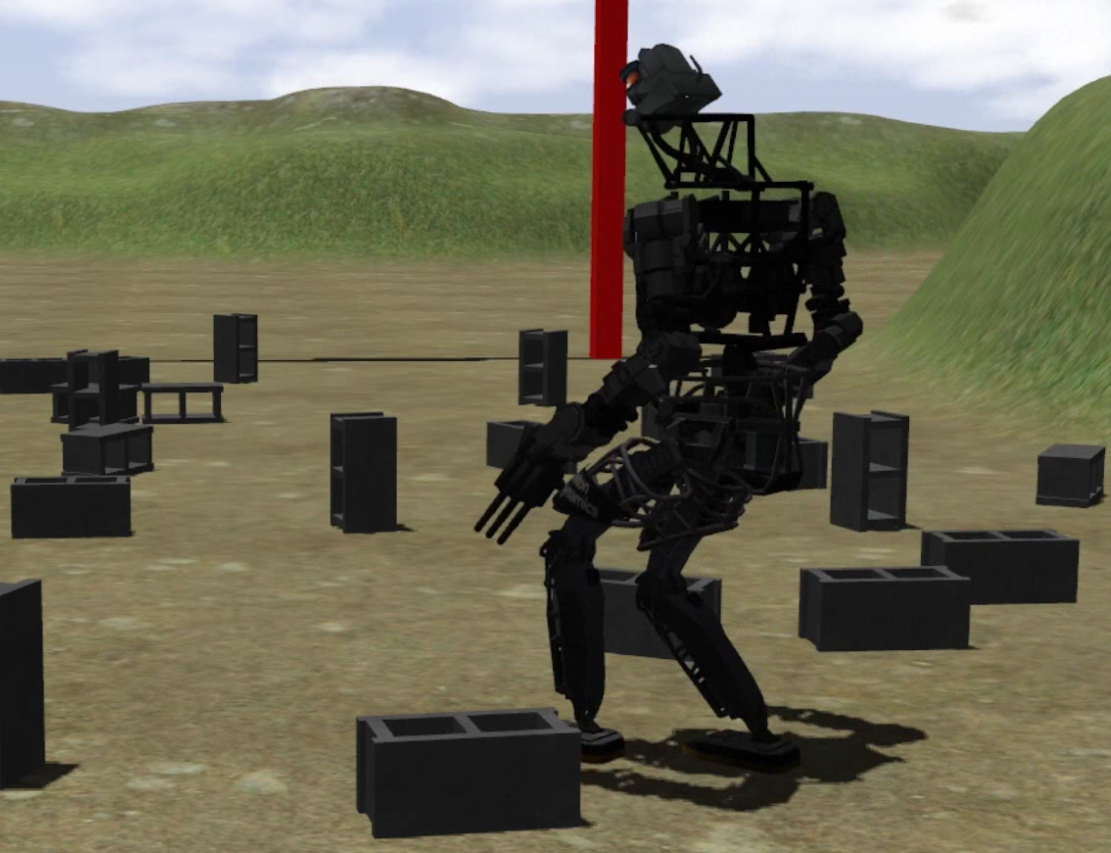
\includegraphics[width=\textwidth]{pics/darpa_walking}
    \caption{Crossing rough terrain}
    \label{fig:vrc_walking}
  \end{subfigure}
  \begin{subfigure}[b]{0.3\textwidth}
    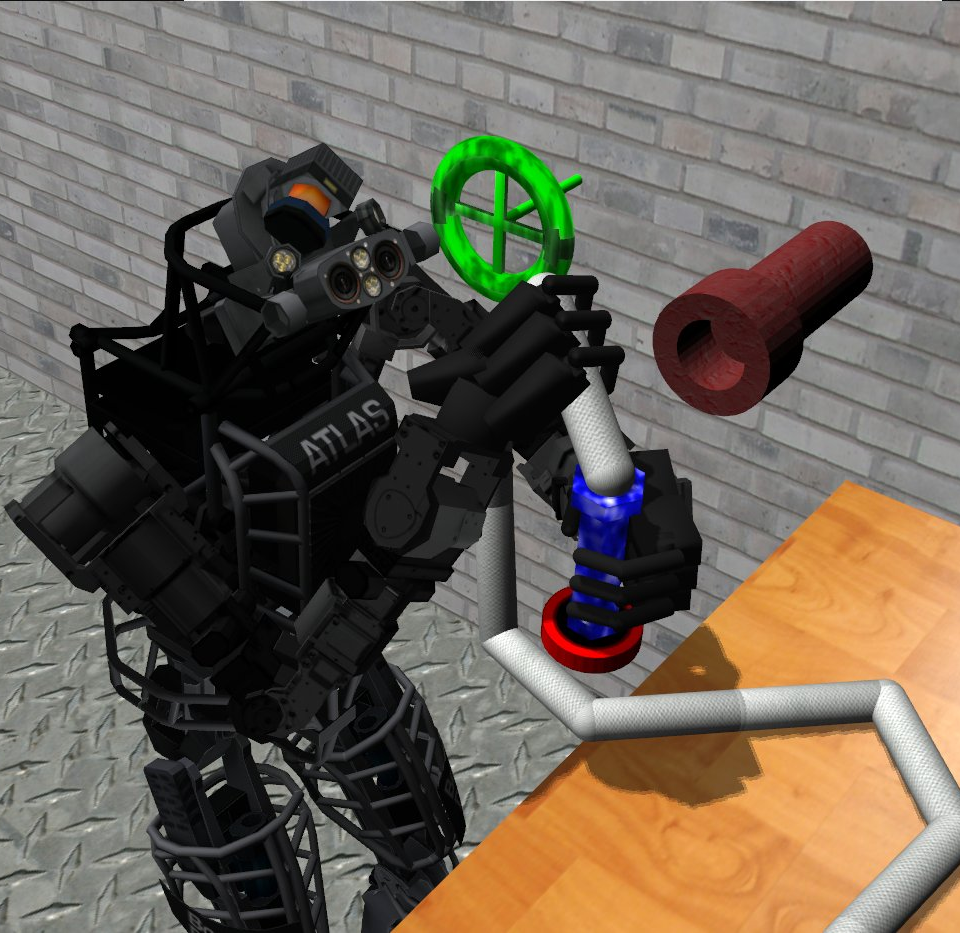
\includegraphics[width=\textwidth]{pics/darpa_hose}
    \caption{Connecting a hose}
    \label{fig:vrc_hose}
  \end{subfigure}
  \caption{Tasks of the Virtual Robotics Challenge~\cite{vrc_pics}}
  \label{fig:vrc}
\end{figure}
The \textit{Virtual Robotics Challenge (VRC)} is a competition by DARPA\footnote{DARPA is the Defense Advanced Research Projects Agency of the USA.} and shows what Gazebo is capable of. The goal of the competition is to solve challenging tasks with a humanoid robot in a simulation. VRC is the first part of the \textit{DARPA Robotics Challenge (DRC)}\footnote{\url{http://www.theroboticschallenge.org}}. DRC aims to spur the development of robots that can operate in a disaster scenario if the situation is too dangerous for humans. An example for such a scenario is the disaster in the Fukushima nuclear power plant after the tsunami in March 2011~\cite{fukushima}. The developed robots should be able to operate in environments made for humans, even if the environment is damaged, and to use tools made for humans, such as screwdrivers and cars. During the competition, the robots act semi-autonomously and are supervised by human instructors. For the challenge, DARPA provides six humanoid robots. The Robots are called \textit{ATLAS} and are developed by Boston Dynamics. The six best teams of VRC receive a ATLAS robot for free. Therefore, ATLAS is the only robot simulated in VRC. However, the participating teams can also build their own robots.
VRC consists of three different tasks~\cite{vrc_rules} showed in Figure~\ref{fig:vrc}. In the first task, the robot has to walk to a car, enter it and drive along a street. The chassis of the car consists of a framework to simplify the entry. On the road, there are obstacles the robot has to avoid. The second tasks tests the walking capabilities of the robot. The robot has to cross slippery and irregular terrain to test balancing and a terrain with obstacles to test perception and footstep planning. The last task is about manipulation. The robot has to connect a hose to a pipe by plugging it in and screwing it down. Afterwards, it has to open a valve. All tasks have randomized parameters, such as the position of obstacles and goals. This tasks show that Gazebo is able to simulate complex situations and environments. The engagement of DARPA shows how important a simulation is for the development and research of cutting-edge technology. Although the technology fostered by DRC is important and useful without doubt, it seems questionable what DARPA as a military agency will use this technology for.


\subsection{RoboCup Simulation Leagues}
\begin{figure}
  \centering
  \begin{subfigure}[b]{0.48\textwidth}
    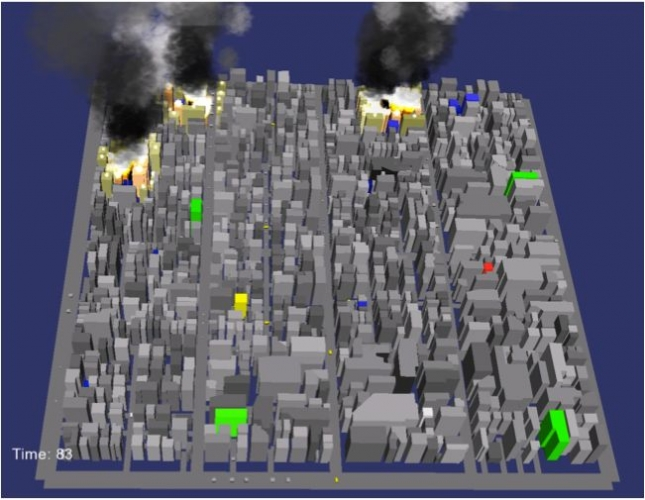
\includegraphics[width=\textwidth]{pics/rescue3d}
    \caption{Agent Competition~\cite{rescue3d}}
    \label{fig:rescue_agent_competition}
  \end{subfigure}
  \begin{subfigure}[b]{0.48\textwidth}
    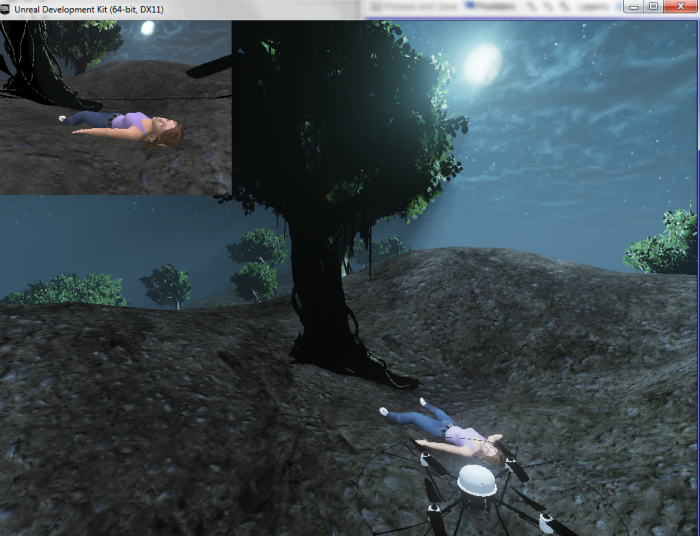
\includegraphics[width=\textwidth]{pics/rescue_vrc}
    \caption{Virtual Robot Competition~\cite{rescue_simulation_league}}
    \label{fig:rescue_vrc}
  \end{subfigure}
  \caption{Rescue Simulation Leagues}
  \label{fig:rescue}
\end{figure}
In the RoboCup competition, there are different simulation leagues. On the one hand, there are the 2D and 3D soccer simulation leagues and on the other hand there are two rescue simulation leagues. In all of those leagues, multi-robot coordination is an important field. This is not surprising because it is much simpler to benchmark multi-robot strategies in a simulation. There is no need to operate real hardware and difficult low level control and sense problems, that are not in the focus of the competition, can be simplified or left out.\\
The \textit{Rescue Simulation League (RSL)} aims to benchmark intelligent software agents and robots in a disaster scenario~\cite{rescue_simulation_league}. RSL is separated into two leagues with focus on different scales. Figure~\ref{fig:rescue} shows snapshots of both simulation. The \textit{Agent Competition} is about a large scale disaster in a city with multiple robot teams. The \textit{Virtual Robot Competition} is about finding victims in a burning house or limited outdoor area with a team of eight robots and one human operator. The operator can give high level commands, such as the area where to look for victims, and is needed to verify the observations of the robots. So, the robots should find and approach victims autonomously and the operator has to confirm the find. The task of the agents include victim-detection, autonomous generation of maps, navigation and multi-agent coordination. In the Agent Competition, there is no realistic robot control and perception necessary. The focus is on the coordination of many heterogeneous agents and taking high level decisions. There are teams of fire brigade, police and ambulance, each with up to 30 simulated agents. Each agent acts autonomously and can communicate with other agents. The tasks of the agents include exploration, scheduling and planning in cooperation with other agents and building of agent teams (e.g. to fight fires more effectively).\\
The soccer simulations of the RoboCup are similarly split in two leagues. In the \textit{2D Soccer Simulation League}, 22 agents in two teams play soccer in a two dimensional environment. A single server called Soccer Server simulates and controls the game with its physics, the actions of the agents and the perception of the agents. Each agent is an autonomous program and communicates with the soccer server to receive noisy sensor data and send action commands to influence the simulation~\cite{soccer_simulation}. The main challenges of the 2D Soccer Simulation League are planning the actions of each agent when playing in offense and reacting on the opponent and predicting his movement when playing in defense. The \textit{3D Soccer Simulation League} features a more realistic simulation. This league fully simulates nine NAO robots per team. Therefore, the low level control and perception are an important part of the challenge~\cite{soccer_simulation_low_level}. This is an important opportunity for the teams participating in the SPL to test their approaches first in the simulation because the SPL also uses the NAO as robot platform. The communication between agents and the Soccer Server in this league is similar to the 2D league. The rules of the league are inspired by the FIFA football rules but have some reasonable extensions~\cite{soccer_rules_3d}. For example a goal directly from the kick off is not allowed and if too many robots are in a small area around the ball, the position of some robots is reset.\\
\begin{figure}
  \centering
  \begin{subfigure}[b]{0.48\textwidth}
    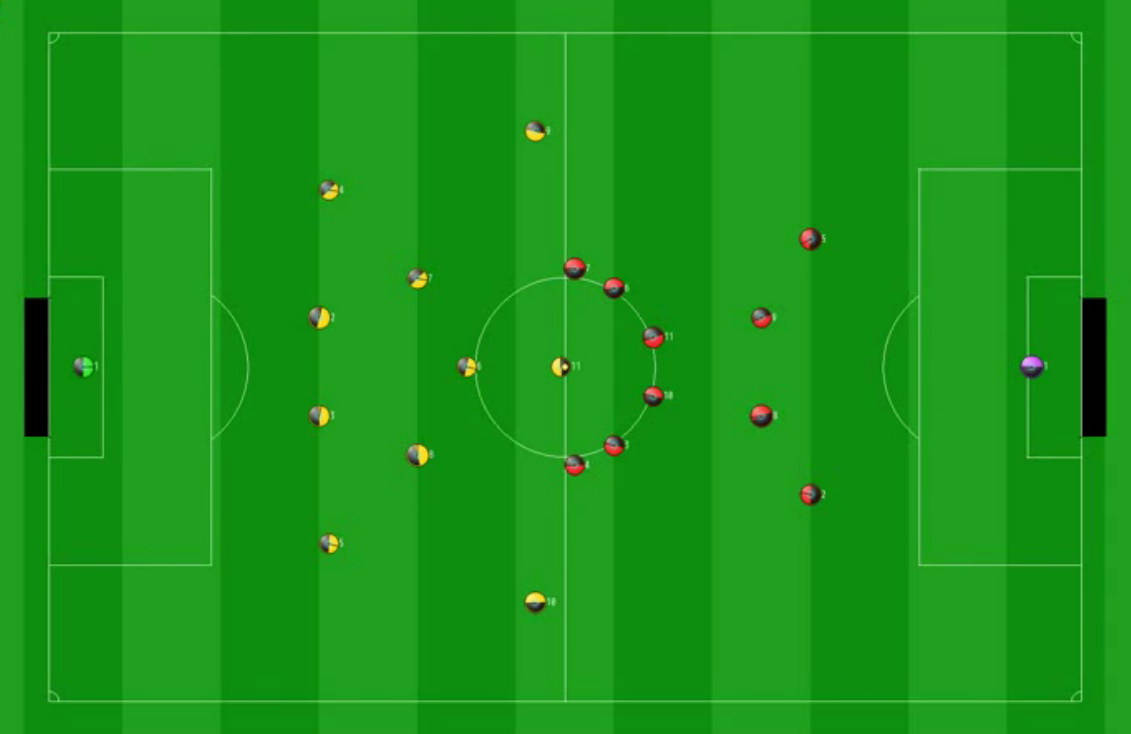
\includegraphics[width=\textwidth]{pics/soccer_sim_2d}
    \caption{2D Soccer Simulation League~\cite{soccer_simulation_2d_pic}}
    \label{fig:soccer_simulation_2d}
  \end{subfigure}
  \begin{subfigure}[b]{0.48\textwidth}
    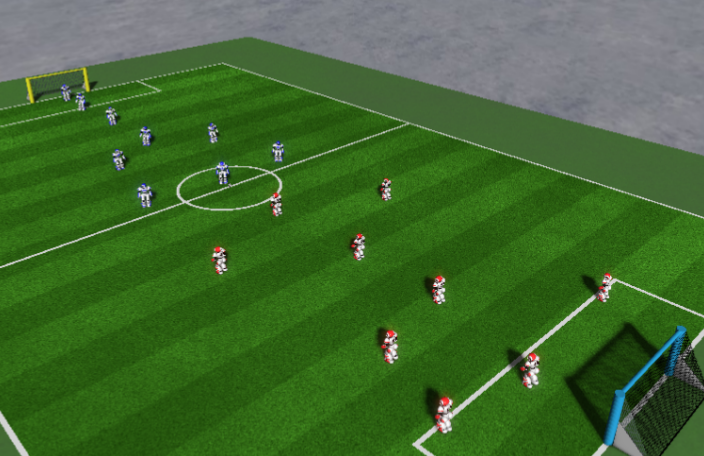
\includegraphics[width=\textwidth]{pics/soccer_simulation_3d}
    \caption{3D Soccer Simulation League~\cite{soccer_simulation_low_level}}
    \label{fig:soccer_simulation_3d}
  \end{subfigure}
  \caption{RoboCup Soccer Simulation Leagues}
  \label{fig:soccer_simulation}
\end{figure}
All simulations we have looked at in this section are similar to the simulation we developed for LLSF. The simulations are important for benchmarking multi-agent systems because the system can be tested with low effort in comparison with real multi-robot systems and some details, such as low level control and perception, can be left out.  Furthermore, the simulations have in common that the evaluation of the whole system can be done by looking at the results and progress of the simulated games. Especially by 2D Soccer Simulation teams, this is used by to do reinforcement learning~\cite{simsoccer_reinforcement_1,simsoccer_reinforcement_2}. Similar as it is possible to improve a real multi-robot system in SPL by improving the performance of the multi-robot system in the 3D Soccer Simulation League~\cite{from_sim_to_real}, we also want to improve our real system by using a simulation.


\subsection{Scene Reconstruction for Fault Analysis}
Some work was already done with Gazebo and Fawkes. Bastian Klingen developed a scene reconstruction for fault analysis in his diploma thesis~\cite{KlingenDA}. The scene reconstruction was primarily made for a mobile robot with a Kinect and a laser range sensors for perception and a gripper arm for manipulation. The task of the robot was to grasp a colored cup on a table. The scenario and the reconstruction are shown in Figure~\ref{fig:klingen}. Because this gripping task involves many components and often fails if a single component fails, a tool was needed to analyze unsuccessful attempts afterwards. This tool reconstructs the scene with the position of the robot, its sensor data and world belief. Therefore the movements, sensor data and belief of the robot have to be logged while performing a grep. The logging was done with MongoDB, which is an Open Source document-oriented database~\cite{mongodb}. Gazebo was used to visualize the perception and belief of the robot to reconstruct the scene. Fawkes was used to control the robot, to log the needed data and to control Gazebo and read the log while reconstructing the scene. Together with the scene reconstruction, Klingen provided a tool to analyze faults to find components that causes the faults. Therefore, he constructed a dependency tree of the components and ordered it in a data-information-knowledge hierarchy.\\
\begin{figure}
  \centering
  \begin{subfigure}[b]{0.38\textwidth}
    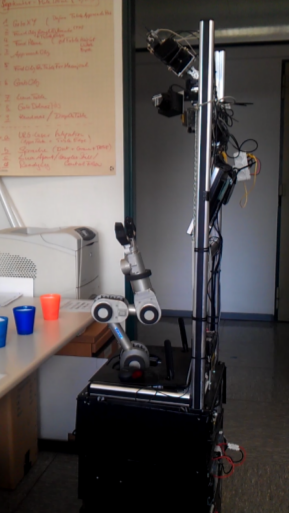
\includegraphics[width=0.7\textwidth]{pics/klingen_real}
    \caption{Grasping a cup in the real scene}
    \label{fig:klingen_real}
  \end{subfigure}
  \begin{subfigure}[b]{0.58\textwidth}
    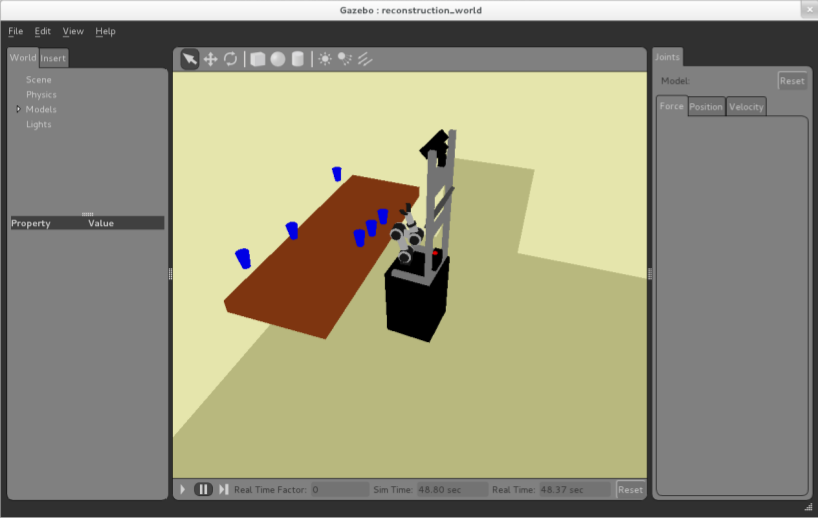
\includegraphics[width=\textwidth]{pics/klingen_sim}
    \caption{Reconstruction in the Gazebo simulator}
    \label{fig:klingen_sim}
  \end{subfigure}
  \caption{Scene Reconstruction for Fault Analysis~\cite{KlingenDA}}
  \label{fig:klingen}
\end{figure}
To establish the communication between Fawkes and Gazebo, Klingen developed a Fawkes plugin that provides the communication objects of the Gazebo API as an aspect. In this thesis, we use this plugin and expand it according to our needs. We also want to reconstruct scenes to analyze them, but in contrast to the work by Klingen we record the scene only in the simulation. We do not record the perception of the robots in the simulation, but we record the movement of all simulated objects and the high level decisions of the agents which can be used to derive the belief of the robot. The motion of the objects in the simulation can be recorded by Gazebo and the agent decisions by logging the results of our rule-based production system CLIPS.

\subsection{Simulation Environment for the Middle Size League}
Another work with Gazebo and Fawkes developed a simulation environment for the MSL~\cite{MultiLevelAbstraction}. This simulation environment became necessary because the field size and the amount of robots per team was increased in MSL. Therefore, testing became more difficult. The work used an early version of Gazebo and Player as interface between Fawkes and Gazebo. On the one hand, it showed that Gazebo is capable of simulating complex robot components that cause problems in other simulators. This was shown for omni-directional wheels and an omni-directional camera. Both devices are non-trivial to simulate and often used in MSL. On the other hand, the work proposed the idea of \textit{multi-level abstraction}. If a robot software contains separate components for steps that are based on each other, it is useful to simulate not only the hardware level, the lowest abstraction level, but also higher abstraction levels. For example if the robot software includes a component that reads an image from a webcam and a component that computes the state of a traffic light from this image, the simulation can provide the simulated image as well as the information about the traffic light. A simulation with multi-level abstraction is able to switch between different abstraction levels. This can be useful to test components on a higher level independent of low level components which can introduce an error or are not finished. Multi-level abstraction has the additional advantage that the components of a higher abstraction level often can be simulated with less computational effort. This makes it easier to run the simulation on a slow computer. However it is not always reasonable to introduce multiple abstraction layers, because some components, such as a collision avoidance, cannot be simulated easily. In this thesis, we also use multi-layer abstraction to be able to test high level components more individually.


\section{Multi-Agent Strategies}
\label{sec:multi_agent_strategies}
In this section, we present our current high level agent approach, which we want to evaluate and improve during the thesis. We also present some advanced multi-agent strategies we might want to use in the future. Our simulation should be able to simulate and evaluate these approaches as well as the current one.

\subsection{Incremental Task-level Reasoning}
Our current implementation of the high-level agent uses the CLIPS rules engine. Our implementation is based on the idea of incremental task-level reasoning~\cite{Incremental}. This means that the agent takes the next best possible action whenever the robot is idle. Simplified, every CLIPS rule represents the choice of taking an action at a specific situation. The situation is encoded in the antecedent of the rule and has to be matched by the fact base. The consequent of the rule includes the execution of the action itself and changes to the fact base to remember the current state. If new perception data is available for the agent or the execution of an action finished or failed, this is asserted as a fact and can therefore cause in the application of some rules to update the belief of the agent in the fact base or to execute the next best action. If more than one action is applicable, the conflict is resolved by choosing the action with the highest priority.\\
The incremental reasoning approach with CLIPS has several advantages. Actions and handling perception can easily be represented by rules which work with the current belief of the agent. The approach is computationally inexpensive, because no costly planning is needed, and it is easy to cope with incomplete knowledge because the agent just takes the next best action and updates the belief if new information is available.\\
Before this thesis, we have been using only two robots. For coordination of these two robots, we use an approach based on roles with additional resource locking. Every agent has a specific role, which determines for which tasks the agent is responsible for and which machines it may use. We have one role for an agent which only produces $P_3$ pucks and delivers them. This agent continuously provides easy points because $P_3$ is the simplest product, which needs only one resource puck (see Figure \ref{fig:llsf_chain}). In the following, we call this role the \textit{$P_3$-role}. A second role is responsible for producing  more complex products, the $P_1$ and $P_2$ pucks. This role can provide a large amount of points, but is more risky because of the higher amount of intermediate steps. We call this role the \textit{$P_1P_2$-role}. Whether the $P_1P_2$-role produces $P_1$ or $P_2$ pucks is determined by the distance between the needed machines to the machine for $P_3$ products. This spacing is necessary because the different robots drive independently and crossing paths can cost much time. Most of the objects in LLSF, such as machines and the delivery zone, can only be used by one robot at a time. Therefore, we implemented a master-slave resource locking mechanism for the agents. If an agent decided to drive to a position, he requests the lock of this position and waits till he receives the lock. Then, he drives there and frees the lock when he leaves the position. The roles are also used for multi-robot coordination in the exploration phase. The roles determine which machine an agent investigates first. After the first machine, the agents continue the investigation of the other machines in the same cycle till all machine types are identified. The agents can pass each other on the cycle.\\
There already is a trivial and fundamentally limited simulation, which is only able to test if the high-level agent basically works. This simulation is implemented within the CLIPS-agent and provides information about the execution of actions and perception results in a trivial way. A few seconds after every action is called from the agent, the action is reported as successful. The perception results match exactly the ground truth published by the Refbox. This is useful to test the behavior of the high-level agent in the best-case scenario. Though, this simulation is only useful to test agent decisions and can therefore not indicate many important real world problems. Furthermore, the simulated situation is not graphically visualized and therefore difficult to evaluate. Testing and evaluate multi-robot coordination is also not possible in this simulation because every agent uses an own simulation and the different time-spans for different actions cannot be taken into account.

\subsection{Marked Based Strategies}
The simulation should be able to test and compare complex multi-robot coordination strategies. An example of such a strategy, which is attractive for our needs and used for orientation in the design process of the thesis, is \textit{Murdoch}~\cite{DissMurdoch}. Murdoch is an auction-based task allocation strategy. It solves a special instance of the \textit{Optimal Assignment Problem}. The Optimal Assignment Problem is to assign $n$ weighted jobs to $m$ workers with non-negative skill ratings $h_{i,j}$ for each worker-job combination. Each worker is capable of doing one job at a time and each job can only be done by one worker. The task is to find the assignment which optimizes the performance, taking into account the weights of the jobs and the skill ratings of the workers to the jobs. The Murdoch method was especially developed 
for multi-robot scenarios. Therefore, it was designed to be able to handle robot failure and communication message loss. If a robot discovers a new task, it becomes an auctioneer and publishes a broadcast message to inform other robots about the task. All robots that are capable of doing the task calculate a metric of how well they probably will perform on the task. The metric is sent as a bid to the auctioneer. Finally, the auctioneer decides after a predefined time interval which robot gets the task and informs this robot. After the allocation, the auctioneer observes the progress of the task and starts a new auction if the robot assigned in the first place fails. This method is to some degree decentralized because the different auctions and metric calculation are not executed by a single robot. However, this approach is not optimal for a set of tasks because every auction only considers a single task. It was shown in~\cite{DissMurdoch} that the method performs well in different multi-agent tasks, such as cooperative manipulation.\\
Murdoch allows a dynamic and situation dependent task allocation and is especially well suited for heterogeneous robots with different abilities. It is also a useful method to allow reallocation of tasks. An agent which is executing a tasks and has already completed a part could change his task if a new task is more important. The agent could simply include the penalty, that it has to cancel a task, and the advantage, that it has from completing the previous task, in his bid for the new task. An example in our domain is a robot which is carrying an intermediate product $S_1$ for the production of a new $P_1$. If an $S_1$ is needed at another machine with higher importance, the robot can change the task. The cancellation of the old task is no problem because the agent can just start a new auction for the old task. Disadvantages of Murdoch are the high demand of communication and the difficulty to detect failures.
